\chapter{}

\section{Zero-energy Signals}

\begin{claim}
    Discrete-time $\text{zero}[n]$ is a zero-energy signal. There are no other zero-energy signals.
\end{claim}

\begin{proof}
    If $x[n] \neq 0$, then $x^2[n] > 0$ for at least one $n$. Thus, $\sum_{n=-\infty}^{\infty} x^2[n] > 0$. Because there's no negative energy, you can't cancel positive energy.
\end{proof}

\section{Energy in Continuous-time}

\begin{claim}
    $\text{zero}(t)$ has zero energy, but there exists other zero-energy signals.
    \[
        x(t) = \begin{cases}
            1 & \text{if } t = 0 \\
            0 & \text{otherwise}
        \end{cases}
    \]
\end{claim}


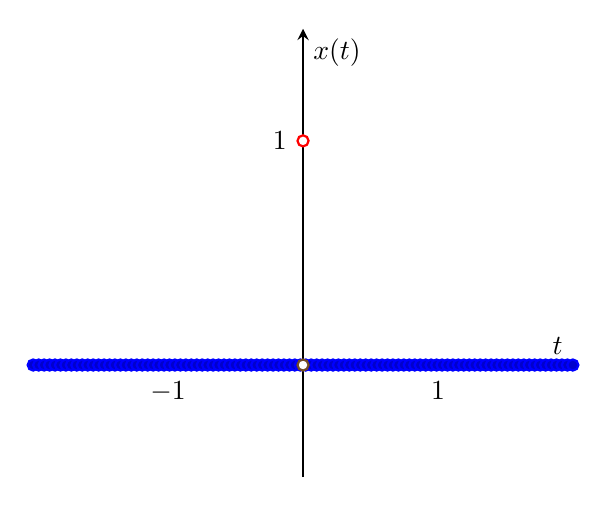
\begin{tikzpicture}
    \begin{axis}[
            xlabel=$t$,
            ylabel=$x(t)$,
            axis lines=middle,
            xmin=-2, xmax=2,
            ymin=-0.5, ymax=1.5,
            xtick={-1,0,1},
            ytick={0,1},
            yticklabels={0,1},
            xticklabels={$-1$,0,$1$},
            samples=100,
            smooth,
            thick
        ]
        \addplot+[domain=-2:2] {ifthenelse(abs(x-0)<0.01, 1, 0)};
        % point at (0,1)
        \addplot+[mark=*,mark options={fill=white}] coordinates {(0,1)};
        % hole at (0,0)
        \addplot+[mark=*,mark options={fill=white}] coordinates {(0,0)};
    \end{axis}
\end{tikzpicture}
\begin{definition}
    [Zero Energy Function]
    We define the \textbf{zero energy function} as
    \begin{align*}
        x_\delta(t) = \begin{cases}
                          1 & \text{if } |t| \leq \Delta \\
                          0 & \text{otherwise}
                      \end{cases}
    \end{align*}
    Then the energy of $x_\delta(t)$ is given by $E_\Delta = 2\Delta$. \\
    So as $\Delta \to 0$, $E_\Delta \to 0$ and $x_\Delta \to 0$.
\end{definition}

\begin{remark}
    \begin{itemize}
        \item A signal of a finite number of impulses will have zero energy.
        \item A signal with a countable infinite number of impulses will have zero energy.
        \item A signal with an uncountable infinite number of impulses will have non-zero energy.
              \begin{itemize}
                  \item Example: $x(t) = \begin{cases}
                                1 & \text{if } t \in \mathbb{Q} \\
                                0 & \text{otherwise}
                            \end{cases}$.
                  \item this may be in the wrong place...
              \end{itemize}
    \end{itemize}
\end{remark}

\begin{vocabulary}
    [Zero Energy Functions]
    If $x(t)$ is a zero-energy function, then we say that $x(t) = \text{zero}(t)$ almost everywhere.
\end{vocabulary}

\begin{vocabulary}
    [Signal Equivalence]
    Say $x(t) = y(t)$ almost everywhere if $x(t) - y(t) = \text{zero}(t)$ almost everywhere.
\end{vocabulary}

\section{Signal Spaces}
\begin{remark}
    \underline{Signal spaces are vector spaces! And signals are vectors!}
\end{remark}

\begin{definition}
    [Signal Addition]
    Given two signals $x, y \in \mathbb+
    {D}$ we can define a new signal $(x+y)$\end{definition}

\begin{remark}
    The addition o two signal sis always a signal
\end{remark}

\section{}